\documentclass[article]{rian_article}

\usepackage{xcolor}
\usepackage{longtable}
%%
% Atenção: Compilar com pdflatex !!!
%%

% Para colocar ao lado use \And para quebrar a linha use \AND
\author{Rian G.S. Pinheiro\\ \email{rian@ic.ufal.br}\And 
        Eric Coelho\\ \email{esc2@ic.ufal.br}}% \And
%         Terceiro Autor\\ \email{terceiro@ic.ufal.br} \AND
%         Quarto Autor\\ \email{quarto@ic.ufal.br} \And
%         Quinto Autor\\ \email{quinto@ic.ufal.br}}

% Autores separados por \&, se mais que 3 usar et al.
\Plainauthor{Rian Pinheiro \& Eric Coelho} %% comma-separated


\title{Algoritmo Genético BRKGA para o Problema de Empacotamento 2D 	Clássico com desempate}
\Plaintitle{Algoritmo Genético BRKGA para o Problema de Empacotamento 2D Clássico com desempate} %% Titulo sem formatação
\Shorttitle{BRKGA com desempate} %% a short title (aparece no topo das páginas)


%% an abstract and keywords
\Abstract{
	O \textit{Problema de empacotamento} (BPP) consiste em armazenar ortogonalmente um conjunto de itens na menor quantidade de caixas possível. A versão clássica assume que os itens têm orientação fixa e não pode haver sobreposição no empacotamento. O caso bidimensional generaliza o problema de empacotamento unidimensional clássico amplamente difundido na literatura, portanto, é da classe \NPhard~.
	Este trabalho apresenta um algoritmo genético de chaves aleatórias viciadas (BRKGA) para o \textit{problema de empacotamento bidimensional} (2BP), considerando os itens alocados com orientação fixa, baseando-se em chaves aleatórias como critério de desempate entre os espaços vazios ao inserir um novo item. O problema tem várias aplicações industriais, como corte, repartição e agendamento, relacionando-se a outros problemas complexos.
}

\Keywords{BRKGA, Two-dimensional Bin Packing, 2BP, Meta-heurísticas}
\Plainkeywords{BRKGA, Two-dimensional Bin Packing, 2BP, Meta-heurísticas} %% sem formatação


%% Informações do Trabalho
\Versao{1}
% \Versao{Final}
\Year{2020}
\Semestre{2}
\Month{Fevereiro}
\Submitdate{\today}
\Disciplina{Pesquisa Operacional}


%%%%%%%%%%%%%%%%%%%%%%%%%% PACOTES %%%%%%%%%%%%%%%%%%%%%%%%%%
\usepackage{amsmath}
\usepackage{bbm}
\usepackage{float}
\usepackage{subfig}
\usepackage{indentfirst}
\usepackage[T1]{fontenc}
\usepackage{url,bm}
\usepackage{textcomp}
\usepackage{graphicx}
\usepackage{amssymb}
\usepackage{anysize}
\usepackage{algpseudocode}
\usepackage{algorithm}
\usepackage{amsthm}
\usepackage{tikz}
\usepackage{enumerate}

%%%%%%%%%%%%%%%%%%%%%%%%% Comandos %%%%%%%%%%%%%%%%%%%%%%%%%%%%
\newcommand{\Cpp}{C\nolinebreak\hspace{-.05em}\raisebox{.4ex}{\tiny\bf +}\nolinebreak\hspace{-.10em}\raisebox{.4ex}{\tiny\bf +}~} 
\newcommand{\NPcom}{$\mathcal{NP}$-completo}
\newcommand{\NPhard}{$\mathcal{NP}$-Difícil}
\newtheorem{teorema}{Teorema}[section]
\floatname{algorithm}{Algoritmo}
\newenvironment{prova}{\begin{proof}[\bf\textsc{Prova.}]}{\end{proof}}



\begin{document}

% Este exemplo foi publicado no SBPO 2015.
\section{Introdução}

O \textit{problema de empacotamento clássico bidimensional} (2BP) consiste em empacotar ortogonalmente um conjunto de $n$ itens em forma de retângulos caracterizados por sua altura $h_{i}$ e largura $w_{i}$, $i \in \{1, 2, 3, ... , n\}$, no menor número possível de caixas homogêneas de altura $H \geq h_{i}$ e largura $W \geq w_{i}$. A quantidade de caixas é ilimitada e os itens não podem ser alocados com sobreposição.

\begin{figure}[hbt]
\centering
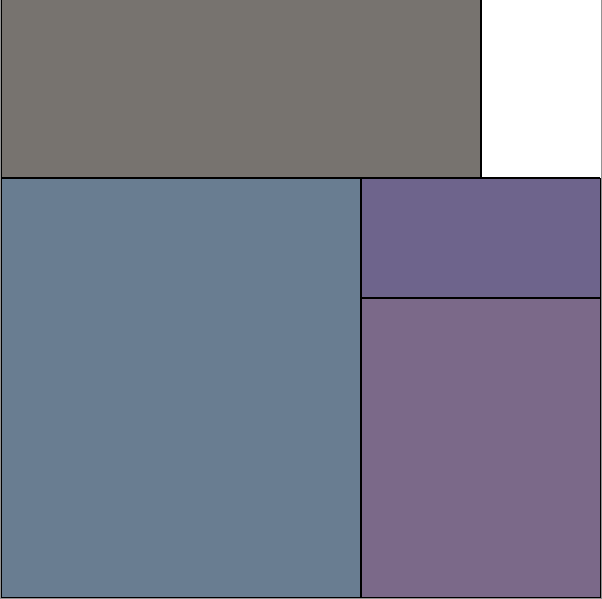
\includegraphics[width=0.3\textwidth]{figs/ex_instance_1.png}\hspace{0.1\textwidth}
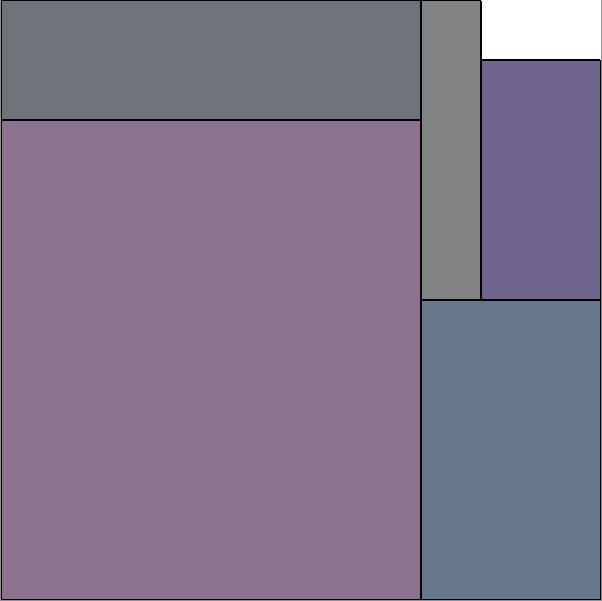
\includegraphics[width=0.33\textwidth]{figs/ex_instance_2.png}
\caption{Exemplo de instância do 2BP.} \label{fig:ex}
\end{figure}

\subsection{Aplicações}
Várias aplicações industriais têm interesse particular no 2BP. Dentre elas, podemos citar aplicações de carregamento de objetos sensíveis em caminhões e aviões, armazenamento de mercadorias, empacotamento de encomendas, reconfiguração dinâmica de hardware e carregamento de paletes. Por exemplo, quando um editor precisa preencher as páginas de um jornal, ele tem que considerar como rearranjar e posicionar os retângulos de textos e propagandas, ou seja, empacotamento de itens em que uma de suas faces deve permanecer obrigatoriamente para cima. Além disso, o problema aparece como subparte de outros problemas mais complexos como os de agendamento, corte e particionamento.\citep{zudio2019}
\section{Algoritmo BRKGA}\label{sec:corte}
O algoritmo genético de chaves aleatórias viciadas (BRKGA) foi introduzido por \citet{resende2011} para problemas de otimização combinatória. Esta meta-heurística é uma variante do algoritmo genético de chaves aleatórias (RKGA) \citep{bean1994}. 
A ideia principal é evoluir uma população codificada em cromossomos. Cada indivíduo é representado por uma sequência de chaves aleatórias ou random-keys, na forma de vetores de números reais no intervalo [0, 1].
O componente chamado decodificador deve ser implementado para cada problema. Este componente deve receber um vetor de random-keys para fornecer uma representação do indivíduo que pode ser avaliada. Para o 2BP, o decodificador é composto de dois componentes: um método de ordenação e um algoritmo guloso para realizar o empacotamento dos itens:

O método de ordenação deve receber um vetor com n random-keys, um para cada item da instância, para fornecer uma permutação de itens. As chaves devem ser ordenadas de modo que o item $a_{i}$ é empacotado antes do item $a_{j}$ se e somente se $k_{i} < k_{j}, {i}, {j} \in \{1, ..., {n}\}$, onde $k_{i}$ e $k_{j}$ são as respectivas random-keys associadas.

\begin{figure}[hbt]
	\centering
	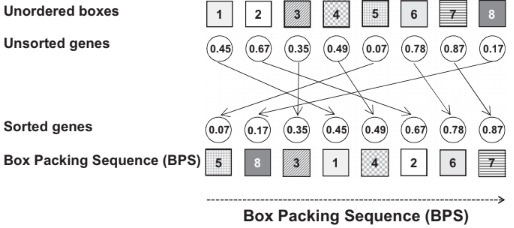
\includegraphics[width=0.8\textwidth]{figs/random_keys.png}
	\caption{Exemplo de BPS \citep{resende2013}.} \label{fig:rand_keys}
\end{figure}

O algoritmo guloso constrói uma solução iterativamente, recebendo uma permutação de inteiros que representa a sequência em que os itens serão empacotados sequencialmente.

Após o processo de ordenação, a permutação associada ao cromossomo do indivíduo é passada como parâmetro de entrada para o algoritmo guloso, denominado Distance to the Front-Top-Right Corner (DFTRC) \citep{resende2013}. Sabendo que uma caixa aberta da solução corrente é uma que contém itens empacotados, para cada iteração {k} do DFTRC, o algoritmo busca por espaços que possam conter o item  $a_{k}, {k} \in \{1, ..., {n}\}$ a ser empacotado. Se nenhuma caixa aberta até o momento pode conter o item, então uma nova caixa é introduzida na solução com $a_{k}$ empacotado. No passo de empacotamento, áreas maximais são utilizadas para modelar o espaço vazio de cada caixa aberta.

\begin{figure}[hbt]
	\centering
	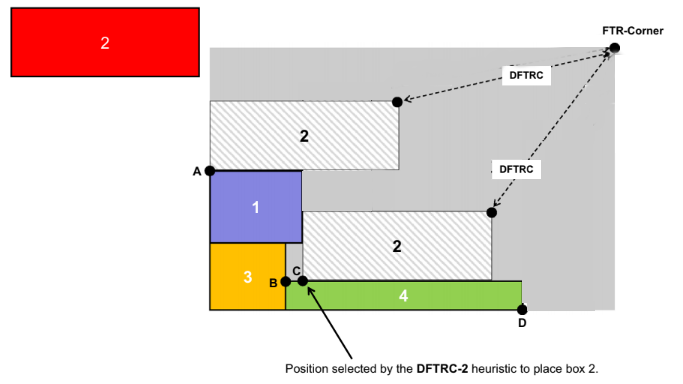
\includegraphics[width=0.8\textwidth]{figs/dftrc.png}
	\caption{Escolha da posição para inserir o item 2.} \label{fig:dftrc}
\end{figure}

Uma área maximal é a maior área retangular possível dentro da caixa aberta que não há itens. Todas as áreas maximais que podem conter o item da iteração corrente são candidatas para a escolha da localização do empacotamento. O DFTRC seleciona a área maximal que maximiza a distância entre o canto superior direito frontal do item para o respectivo canto superior direito frontal da caixa.

Caso haja empate entre as áreas maximais, um segundo vetor de random keys é utilizado para selecionar entre as duas melhores áreas maximais.

\begin{center}
$TB_{i} = \begin{cases}\texttt{Área 1, se random-key}_{n + i} \leq 1/2\\
				\texttt{Área 2, se random-key}_{n + i} > 1/2\end{cases}$
\end{center}
\begin{figure}[hbt]
	\centering
	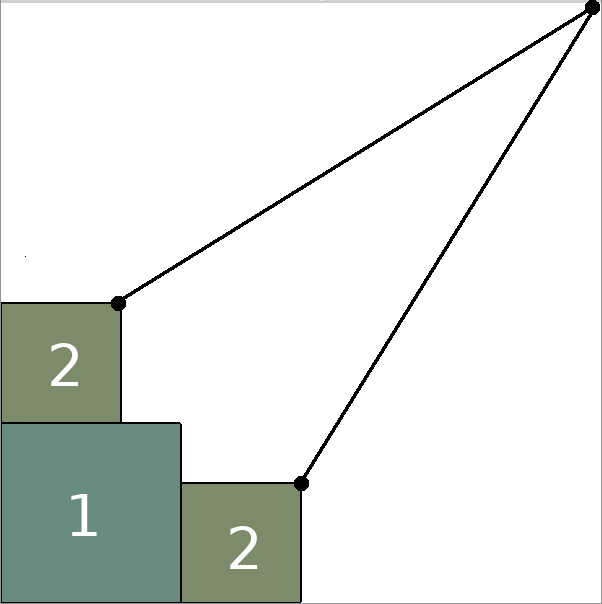
\includegraphics[width=0.5\textwidth]{figs/tie_breaker.png}
	\caption{Exemplo de empate entre espaços maximais.} \label{fig:empate}
\end{figure}

O Algoritmo~\ref{alg:const} apresenta a visão geral do procedimento de empacotamento.

\begin{algorithm}[hbtp]
\caption{Placement}
\label{alg:const}
\begin{algorithmic}[1]
\footnotesize
\Procedure{Placement}{$BPS,TB$}
	\State{Inicialize $B$ com as caixas abertas}
	\State{Inicialize $NB$ com o número de caixas abertas}
	\For{$i \in \{1, ..., {n}\}$}
		\State{$BoxToPack \gets BPS\{i\}$}
		\State {$SelectedBin \gets 0$}\Comment{Nenhuma caixa escolhida}
		\For{$k \in \{1, ..., {NB}\}$}
			\State{$BestEMSList \gets$ \textsc{DFTRC}($k, BoxToPack$)}\Comment{O DFTRC retorna os espaços para o empacotamento}
			\If{$BestEMSList > 0 $}\Comment{Encerra o loop ao encontrar uma solução}
				\State {$SelectedBin \gets k$}
				\State \textbf{break}
			\EndIf
		\EndFor
		\If{$BestEMSList \neq \emptyset$}
			\State{$EMSselected \gets$ \textsc{EMSSelector}($TB_i, BestEMSList$)}\Comment{Aplica o critério de escolha para o desempate}
		\Else
			\State{$NewBin \gets NB + 1 $}\Comment{Abre uma nova caixa e insere o item}
			\State{$B \gets B \cup {NewBin} $}
			\State{$NB \gets NB + 1 $}
			\State{$EMSSelected \gets NewBin_0 $}
		\EndIf
		\State{Calcula a posição do item na caixa a partir de $EMSSelected$}
		\State{\textsc{DifferenceProcess}($SelectedBin, BoxToPack$)}\Comment{Realiza o procedimento DP de \citet{chan1997}}
	\EndFor
\EndProcedure
\end{algorithmic}
\end{algorithm}

\subsection{Função Objetivo}
A função objetivo do problema de empacotamento é o próprio número de caixas abertas. Porém, diversas soluções utilizam a mesma quantidade de caixas, portanto, a quantidade de caixas utilizadas pode não avaliar bem o potencial de melhora de uma solução.
Para resolver este problema, \citet{resende2013} propôs uma função
objetivo alternativa (aNB), que diferencia as soluções com a mesma quantidade de caixas. A função aNB utiliza a carga de espaço ocupado pela caixa que estiver com menor carga. Assim, o potencial de melhora de uma solução é dado através de uma fração no intervalo $]0, 1[$. Dadas duas soluções que compartilham o mesmo número de caixas, a que apresenta a caixa com
menor carga será a que tem mais potencial para melhora.

\begin{center}
$aNB = NB + \dfrac{LeastLoad}{BinCap}$
\end{center}


\section{Experimentos Computacionais}
A base de testes utilizada neste trabalho é composta por 500 instâncias do 2BP detalhadas em \citet{martello1998}. As instâncias são organizadas em 10 classes com 10 instâncias para cada quantidade de itens ${n} \in \{20, 40, 60, 80, 100\}$. Esta base se trata de uma extensão das instâncias propostas em \citet{wang1987}.

\subsection{Ferramentas}\label{sec::ferramentas}

O BRKGA proposto foi implementado utilizando a linguagem de programação C++11, e foi compilado com o GCC do GNU Compiler Collection. O ambiente computacional utilizado em todos os testes neste trabalho consiste de um desktop munido da seguinte configuração: processador AMD FX-6300 @3.5 GHz, 8 GB de memória RAM e sistema operacional Ubuntu 18.04. A Tabela~\ref{tab:params} relaciona os parâmetros calibráveis do BRKGA com os respectivos valores.

\begin{table}[htb]
	\caption{Parâmetros do BRKGA}
	\label{tab:params}
	\centering
	\footnotesize
	\begin{tabular}{|c|c|}
		\hline
		Componente               &Configuração \\ \hline
		Critério de parada       &200 gerações	 \\ \hline
		Tamanho da população     &$P_{max} = 30 \times {n}$	 \\ \hline
		Fração TOP               &$\epsilon = 0,1$	 \\ \hline
		Fração BOT               &$\omega = 0,15$	 \\ \hline
		Taxa de elitismo         &$\rho = 0,7$	 \\ \hline
	\end{tabular}
\end{table}


\subsection{Resultado}
\begin{longtable}{|l|c|c|c|c|}
	\caption{Resultados}
	\label{tab:result} \\
	\hline
	\multicolumn{1}{|c|}{\textbf{Class}} & \multicolumn{1}{c|}{\textbf{Bin size}} & \multicolumn{1}{c|}{\textbf{n}} & \multicolumn{1}{c|}{\textbf{aNB \citep{resende2013}}} &  \multicolumn{1}{c|}{\textbf{aNB com desempate}}\\ \hline 
	\endfirsthead
	1 & 10 x 10 & 20 & 7.10 & 7.10 \\ \hline
	&  & 40 & 13.40 & 13.40 \\ \hline
	&  & 60 & 20.00 & 20.00 \\ \hline
	&  & 80 & 27.50 & 27.50 \\ \hline
	&  & 100 & 31.70 & 31.70 \\ \hline
	2 & 30 x 30 & 20 & 1.00 & 1.00 \\ \hline
	&  & 40 & 1.90 & 1.90 \\ \hline
	&  & 60 & 2.50 & 2.50 \\ \hline
	&  & 80 & 3.10 & 3.10 \\ \hline
	&  & 100 & 3.90 & 3.90 \\ \hline
	3 & 40 x 40 & 20 & 5.10 & 5.10 \\ \hline
	&  & 40 & 9.40 & 9.40 \\ \hline
	&  & 60 & 13.90 & 13.90 \\ \hline
	&  & 80 & 18.90 & 18.90 \\ \hline
	&  & 100 & 22.30 & 22.30 \\ \hline
	4 & 100 x 100 & 20 & 1.00 & 1.00 \\ \hline
	&  & 40 & 1.90 & 1.90 \\ \hline
	&  & 60 & 2.50 & \textbf{2.40} \\ \hline
	&  & 80 & 3.10 & \textbf{3.20} \\ \hline
	&  & 100 & 3.70 & \textbf{3.80} \\ \hline
	5 & 100 x 100 & 20 & 6.50 & 6.50 \\ \hline
	&  & 40 & 11.90 & 11.90 \\ \hline
	&  & 60 & 18.00 & 18.00 \\ \hline
	&  & 80 & 24.70 & 24.70 \\ \hline
	&  & 100 & 28.10 & 28.10 \\ \hline
	6 & 300 x 300 & 20 & 1.00 & 1.00 \\ \hline
	&  & 40 & 1.60 & 1.70 \\ \hline
	&  & 60 & 2.10 & 2.10 \\ \hline
	&  & 80 & 3.00 & 3.00 \\ \hline
	&  & 100 & 3.30 & 3.40 \\ \hline
	7 & 100 x 100 & 20 & 5.50 & 5.50 \\ \hline
	&  & 40 & 11.10 & 11.10 \\ \hline
	&  & 60 & 15.80 & 15.80 \\ \hline
	&  & 80 & 23.20 & 23.20 \\ \hline
	&  & 100 & 27.10 & 27.10 \\ \hline
	8 & 100 x 100 & 20 & 5.80 & 5.80 \\ \hline
	&  & 40 & 11.30 & 11.30 \\ \hline
	&  & 60 & 16.10 & 16.10 \\ \hline
	&  & 80 & 22.40 & 22.40 \\ \hline
	&  & 100 & 27.80 & 27.80 \\ \hline
	9 & 100 x 100 & 20 & 14.30 & 14.30 \\ \hline
	&  & 40 & 27.80 & 27.80 \\ \hline
	&  & 60 & 43.70 & 43.70 \\ \hline
	&  & 80 & 57.70 & 57.70 \\ \hline
	&  & 100 & 69.50 & 69.50 \\ \hline
	10 & 100 x 100 & 20 & 4.20 & 4.20 \\ \hline
	&  & 40 & 7.40 & 7.40 \\ \hline
	&  & 60 & 10.00 & 10.00 \\ \hline
	&  & 80 & 12.80 & 12.80 \\ \hline
	&  & 100 & 15.80 & 15.80 \\ \hline
\end{longtable}

A Tabela \ref{tab:result} apresenta a média de caixas obtidas para as instâncisa de cada Classe ${i}$ da solução encontrada na literatura \citep{resende2013}, juntamente com a solução do BRKGA proposto.
Observa-se que o algoritmo BRKGA com desempate encontra o valor equivalente em todas as instâncias com exceção das médias de {n} = 60, 80 e 100 da classe 4, onde o resultado somente foi melhor no caso {n} = 60.

\section{Conclusão}
Este trabalho aplicou a heurística BRKGA para o problema clássico de empacotamento bidimensional, sem considerar a rotação dos itens. O algoritmo é baseado na meta-heurística BRKGA, e utiliza um algoritmo guloso para empacotar os itens. Através de um conjunto de 500 instâncias, as quais compõem a base de teste padrão para vários trabalhos encontrados na literatura, o BRKGA com desempate foi comparado com o BRKGA \citet{resende2013}. Os experimentos mostraram que o BRKGA proposto aliado com o critério de desempate obtém vários resultados equivalentes ou melhores aos reportados.

Para trabalhos futuros com relação a meta-heurística, pode-se pensar em novos métodos que permitam encontrar soluções mais próximas do limite inferior, e a melhora no resultado das instâncias que foram afetadas.


\bibliography{refs2}
\end{document}
